%! Author = denis
%! Date = 15/09/2025



% Slide 2
\begin{frame}{Internet das Coisas - IoT: Conceitos Básicos}
    Definições:

    \begin{columns}[c] % 'c' centraliza verticalmente
        % --- Coluna do texto (esquerda) ---
        \column{0.55\textwidth}
        \small
        \textit{"A Internet das Coisas é um paradigma no qual objetos físicos do mundo real são conectados à internet, podendo identificar-se, comunicar-se e interagir com outros dispositivos e sistemas."}
       
        % --- Coluna da imagem (direita) ---
        \column{0.45\textwidth}
        \begin{center}
            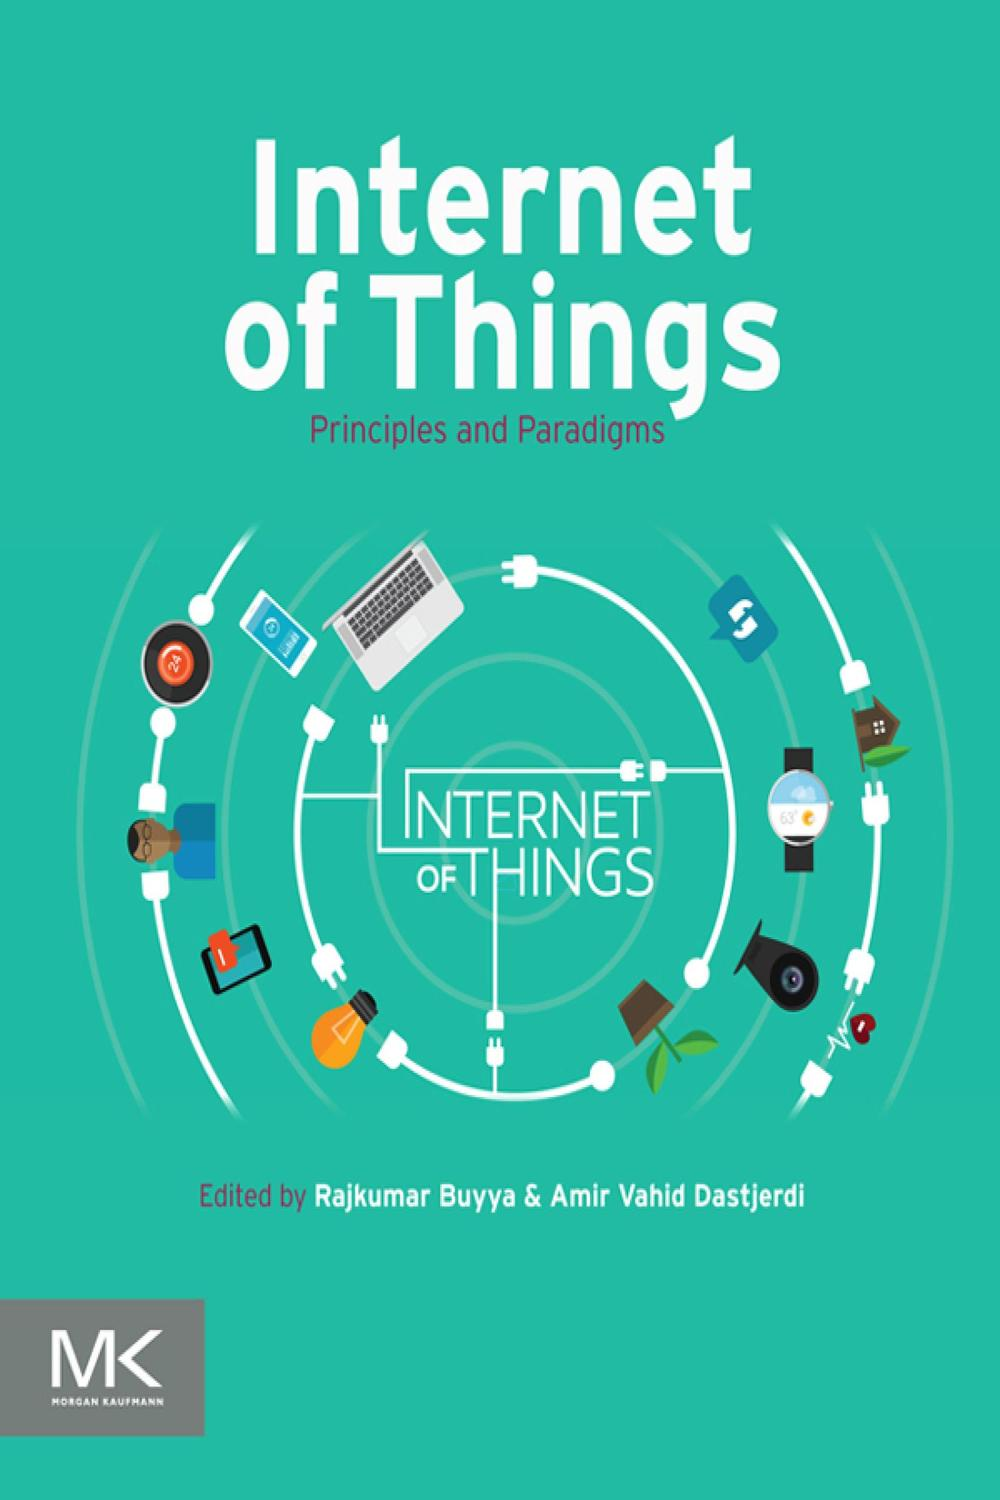
\includegraphics[width=0.35\textwidth]{images/book_1.jpg}
            \label{fig:Internet of Things: Principles and Paradigms}
        \end{center}
    \end{columns}
    
    \begin{columns}[c] % 'c' centraliza verticalmente
        % --- Coluna do texto (esquerda) ---
        \column{0.55\textwidth}
        \small
        \textit{"A Internet das Coisas consiste em objetos conectados que possuem sensores, software e conectividade de rede, permitindo coletar dados e interagir com o ambiente físico."}
       
        % --- Coluna da imagem (direita) ---
        \column{0.45\textwidth}
        \begin{center}
            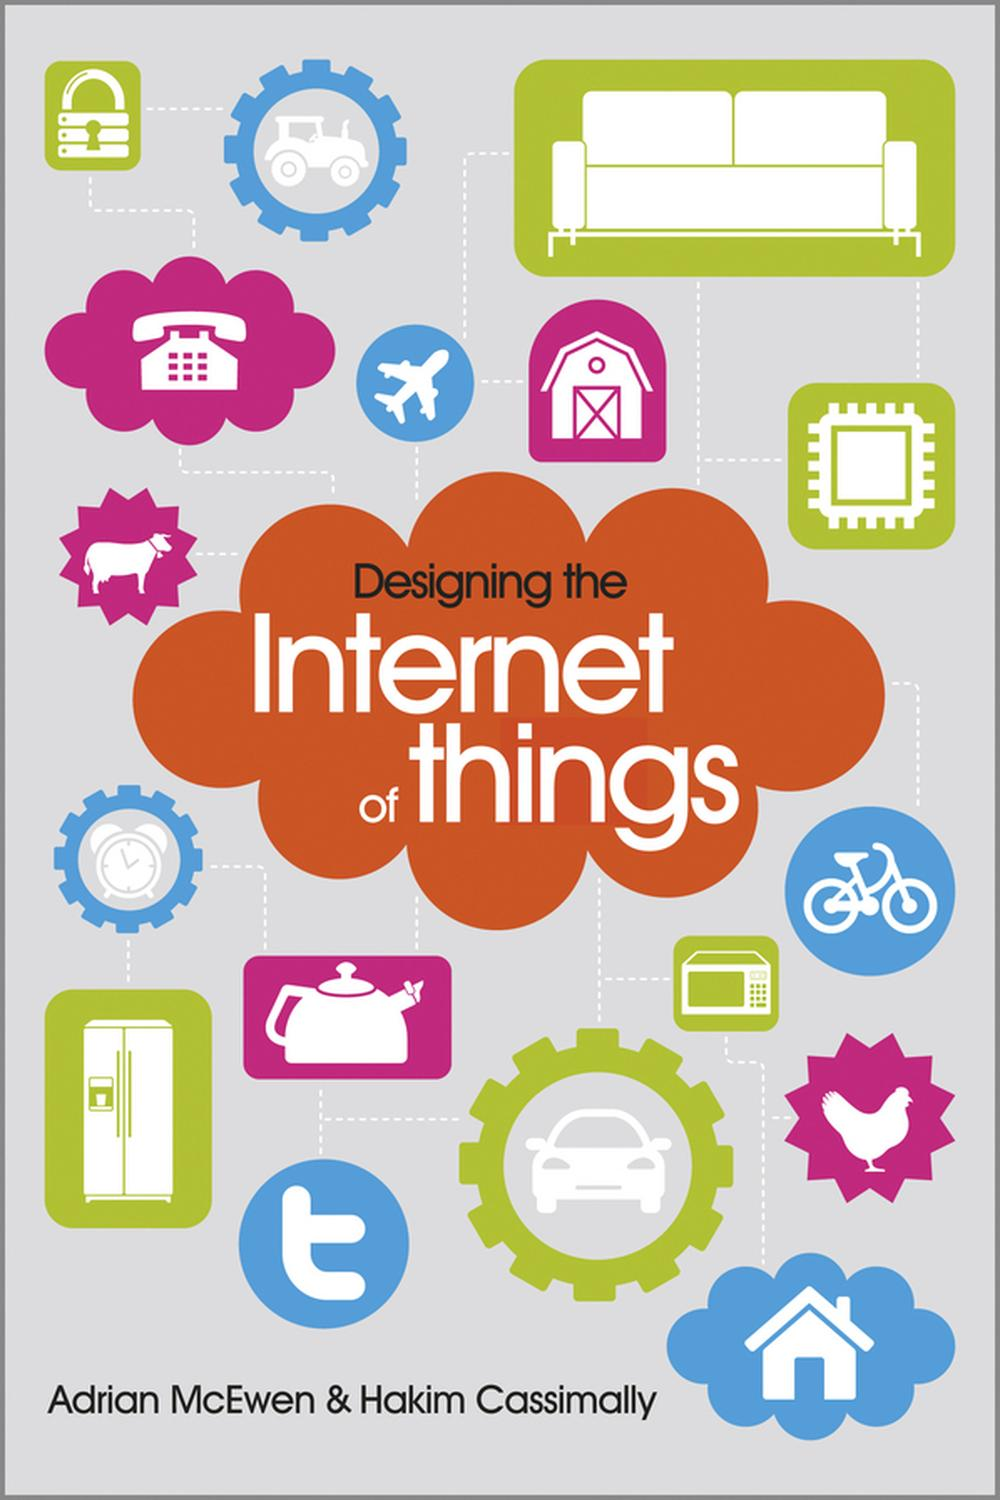
\includegraphics[width=0.35\textwidth]{images/book_2.jpg}
            \label{fig:Designing the Internet of Things}
        \end{center}
    \end{columns}
\end{frame}
